\section{Introduction} \label{sec:introduction}

A key challenge in evolutionary biology is understanding how complex phenotypic traits and new genetic information arise.
Among other factors, theory identifies gene duplication as a major contributor to biological diversity and complexity \citep{Zhang2003,Otto2000,Wagner2008,Crow:2006role,Magadum:2013wu,Metz:chromosomeDuplication1947,Hu:2010ea,Castellanos2024,Lynch2000b,Lynch2003}.
While comparative genomic studies have provided an increasingly detailed account of duplication events shaping genetic and phenotypic traits in nature \citep{Zhang2014,teichmann_structural_1998,Teichmann:2004cz,DuBose2024,Voordeckers2012,Pougach2014,Moore2003}, ambiguities remain in bridging these findings with explicit, process-based models of evolutionary dynamics \citep{Welch2016}.
In particular, it remains difficult to gauge the importance of adaptive processes like neo-functionalization and dose effects versus contingent processes driven by drift and historical constraint \citep{Innan2010,Zhang:2003fw,Kuzmin2022}.

% Mirroring larger questions around the adaptive framings of evolutionary origins of biological complexity, gene duplication is thought to lead to increased complexity both by increasing opportunities for the accumulation of contingent complexity (``sub-functionalization'') and by facilitating adaptive discovery of beneficial novel traits (``neo-functionalization'').
In modern evolutionary biology, experimental approaches have become an important complement to retrospective studies, helping to establish causality in evolutionary dynamics \citep{Kawecki2012,Elena2003}.
Notable experimental evidence using microbial populations has established the adaptive significance of duplicative dose effects \citep{Tong2025,Dhar2014,Nsvall2012}.
Also notable is recent \textit{in vivo} experimental work by \citet{mihajlovic2025direct}, who apply a directed evolution approach using fluorescence-activated cell sorting to compare the rate of adaptive evolution for between \textit{E. coli} strains differing in copy count for genes encoding fluorescing protein coGFP.
Over five rounds of mutagenesis, amplification, and selection, Mihajlovic et al. demonstrate that fluorescence phenotypes in double-copy populations exhibit greater robustness under mutation, but they do not find evidence of faster adaptation in double-copy populations vis-a-vis fluorescence intensity.
As the authors highlight, though, achieving the work within their model system required trade-offs in using mutation rates and selection pressures differing significantly from those typical in natural evolution.

The theme of evolution of complexity has drawn notable contributions, in particular, from experiments incorporating digital model systems \citep{Fortuna2022}.
While lacking in realism and richness compared to work with biological organisms, \textit{in silico} approaches offer complementary capabilities in supporting principled definitions of complexity \citep{Adami2002}, fast throughput spanning thousands of generations, and flexible exploration of arbitrary counterfactuals \citep{langton1989artificial}.
In this work, digital systems allow us to systematically enable or disable duplications, supporting direct comparisons of evolutionary outcomes.
Insight may also be gained from tracing the fate of duplicated sites, given the availability of exhaustive mutational histories.

\begin{figure}[!ht]
\centering
% https://docs.google.com/presentation/d/109vfeK_lHSsE0q7Iz7tzl9sDxnP8jyOF2gJ-v85pgL8/edit?usp=sharing
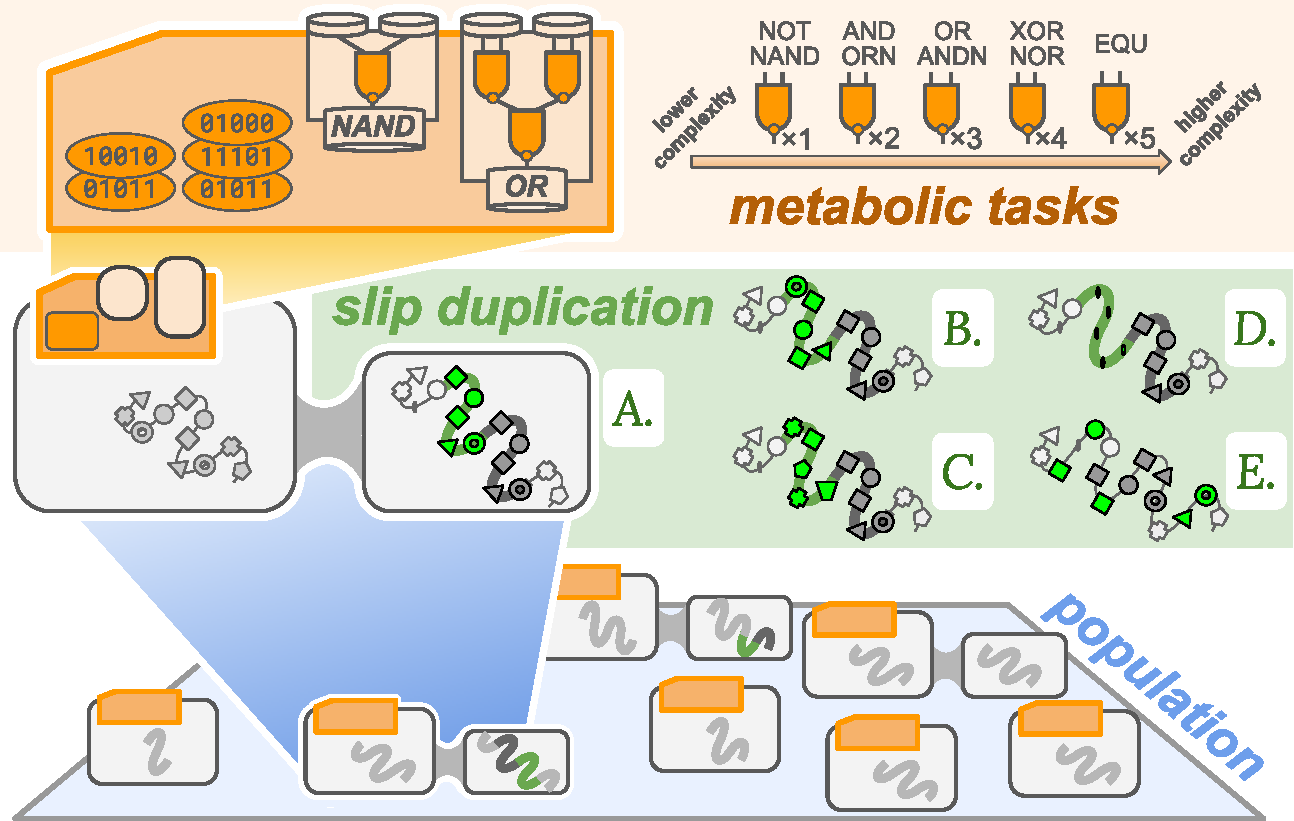
\includegraphics[width=\linewidth]{imgs/GeneDupeOps.pdf}

\vspace{2ex}

\caption{%
\textbf{Genome replication and phenotypic traits in Avida.}
\footnotesize
Self-replicating computer programs serve as digital model organisms (bottom panel).
Organisms comprise virtual stacks and registers used to store binary values and pointers within a genome of program instructions used to track instruction execution and copying.
Competition to survive and reproduce occurs within a limited-capacity population.
Replication activity can be accelerated by carrying out available ``metabolic'' input/output tasks (top panel).
These tasks vary in complexity with respect to the number of NAND operations required to perform them.
An organism's metabolic ``phenotype'' arises from the expression of its genetic code.
Genetic code copied from parent to offspring may be subject to point mutations, which change the individual instruction values, and slip mutations, which introduce or remove many instructions all at once (slip inserts shown as bright green).
Reported experiments compare five alternate variants of slip mutation:
A) \textit{Slip-duplicate}, an exact duplication is inserted adjacent to the target segment;
B) \textit{Slip-scramble}, shuffled duplication is inserted directly after the target segment;
C) \textit{Slip-random}, random instructions are inserted directly after the target segment;
D) \textit{Slip-NOP}, neutral nop-X instructions are inserted directly after the target segment; and
E) \textit{Slip-scatter}, randomly-drawn instructions are inserted at random throughout the genome.
}
\label{fig:slip_mut_variants}
\end{figure}


Here, we investigate the role of adaptive innovation in the relationship between gene duplication and the evolution of complexity using the Avida digital evolution platform.
This system allows evolution experiments to be conducted using populations of self-replicating computer programs, operating as digital ``model organisms'' \citep{Ofria:2009avida};
owing to heritable variation in replication rate introduced by copy errors, evolution by natural selection unfolds within these populations \citep{pennock2007models}.
Among other early work with Avida, Lenski \textit{et al.} established a useful framework for quantifying the complexity of phenotypic traits evolved by Avida organisms, by counting the minimum number of necessary substeps to accomplish a task of interest \citet{Lenski2003Evolutionary}.
Applying this lens to a phenotype  (``EQU'') comprising a large number of substeps, controlled experiments and step-by-step lineage analyses demonstrated that simple traits could provide building blocks for EQU --- and, in fact, amounted to necessary prerequisites for the evolution of complex traits.
Other work with Avida has yielded wide-ranging contributions shedding light on selection's influence on information-theoretic measures of genome complexity \citep{Adami2000Evolution}, co-evolutionary pressures toward complex phenotypic traits \citep{Zaman2014Coevolution}, and the abundance of genetic encodings for complex phenotypes \citep{Fortuna2017GenotypePhenotype}.

To determine the role of novel adaptations in complexity arising from gene duplication, we independently assessed the influence of slip-duplication mutations on both genetic and phenotypic complexity.
We measured genetic complexity by counting the program instructions contributing to an organism's fitness.
For phenotypic complexity, we used the minimal quantity of computational substeps necessary to recreate exhibited behaviors \citet{Lenski2003Evolutionary}.
We find that gene duplication facilitates adaptive evolution of phenotypic traits, with this adaptive benefit appearing exclusively for complex traits.
Moreover, we show genome sites encoding complex phenotypic traits to be disproportionately localized within slip-duplicated regions.
Genetic complexity, by comparison, did not appreciably respond to gene duplications.
Our results therefore contrast with perspectives on biological complexity according lesser significance to the role of adaptive innovation \citep{Lynch2000,Beslon2021,Lynch2007}.
%, which expect changes more strongly associated with subfunctionalization of existing traits \citep{TODO}.

Figure \ref{fig:slip_mut_variants} provides a schematic overview of the experiments conducted in our work.
All experiments comprised well-mixed populations with a carrying capacity of 3,600 Avida organisms.
To supply adaptive potential, we adopted an framework developed by Lenski \citet{Lenski2003Evolutionary} to define a set of nine advantageous phenotypic traits.
Each trait corresponds to a possible logical transform on available binary inputs.
Under this scheme, organisms producing correct output values for a task benefit by accelerating their genome evaluation (and, thus, also their self-replication), analogously to a metabolic process.
Formally, ``substeps'' necessary to carry out each task may be quantified in terms of the minimum number of NAND operations necessary to carry it out \citep{Lenski2003Evolutionary}.%
\footnote{
Computer architecture theory considers NAND as a fundamental basis operation, since all other logic can be derived from compositions of NAND operations \citep{mano1997logic}.
}
As seen in Figure \ref{fig:slip_mut_variants}, the most complex function (EQU) requires five NAND operations while the simplest (NAND and NOT) require only one.
% In other work, EQU has been shown to require at least around 20 constituent genome sites, with many possible longer ways to accomplish EQU \citep{Lenski2003Evolutionary}.

Avida organisms replicate asexually by copying their genome one locus at a time.
In addition to a baseline point mutation rate, our experiments
% implemented a series of mutation operators to systematically isolate aspects of gene duplication and tease apart which factors promote evolvability.
modeled gene duplication events using ``slip mutation'' processes analogous to replication slippage \citep{bzymek_instability_2001}.
Under baseline conditions, these slip mutations allow arbitrary segments of program content to be duplicated or excised.
% It is also possible that ``side effects'' of gene duplication may contribute to adaptive evolution, such as effects in increasing effective mutation rate, localized clustering of sequence changes, and increases in genome length.
%Due to their inherent co-occurrence, it is not obvious how to disentangle these aspects of gene duplication in field or laboratory studies.
As overviewed in Figure \ref{fig:slip_mut_variants}, we also tested a series of mutation operators isolating particular functional effects of gene duplication, in order to tease apart causality in greater detail.
Experiments began with 100-site genomes.
To control for the effects of genome length, we also included trials with longer 1,000-site genomes, which was near the upper extreme of genome lengths observed over the course of slip-duplication experiments.

% \subsection{Major Results}

% We found local slip mutations that duplicate intact regions to be the most effective configuration of gene duplication in facilitating evolution on the Logic-9 task set within the Avida platform.
% In particular, we found that --- compared to control experiments with long genome sizes --- gene duplication uniquely promoted the evolution of complex adaptive traits.
% We further found that the raw material created by slip duplication plays a potentiating role in the evolution of complex traits.
% Specifically, we identified that slip-duplicated regions are significantly more likely to serve as coding sites for new traits when they first appear.
% Consistent with expectations under neofunctionalization theory, however, we did not observe potentiation effects of slip duplication on the evolution of simple traits, only traits that were facilitated by multiple building block components.

% Finally, we assessed the consequences of slip duplication on genome architecture.
% One hypothesis is that gene duplication would promote genetic brittleness by increasing genome length and accelerating growth in contingent complexity, as newly redundant genetic material specializes over time.
% Contrary to this possibility, we found that active coding sites grew as a rate similar to control experiments.
% However, we observed that slip duplications produced a significant increase in the accumulation of coding material, when active and vestigial sites are considered together.
% To understand this phenomenon, we tested the immediate effects of slip duplication on genome brittleness.
% We found that, on average, fitness-neutral slip duplications decreased, rather than increased, the number of information-baring sites in a genome.
% These results align with our observed increase in vestigial coding material in genomes.
% These brittleness-reducing effects appear to be counteracted by other factors, resulting in a similar overall trajectory of genome information content between the slip-duplication and control treatments.

%%%%%%%%%%%%%%%%%%%%%%%%%%%%%%%%%%%%%%%%%%%%%%%%%%%%%%%%%%%%%%%%%%%%%%%%%%

% In our experiment, we used the capabilities of the digital evolution platform to compare evolutionary outcomes in terms of the complexity of traits evolved when mutational processes that duplicated genome regions were included, excluded, as well as a .

% Gene duplication events are widely recognized as a key factor in the evolution of organismal complexity.
% Mirroring broader contrasts between adaptation- versus contingency-driven hypotheses for the evolutionary origins of biological complexity, gene duplication outcomes are typically framed in terms of neo- and sub-functionalization scenarios.
% In the former, duplicated genetic material catalyzes novel functionality; in the latter, it is co-opted to elaborate existing functionality.
% Examples of both scenarios are widespread in natural history, but practical constraints have limited direct experimental investigation of the relationship between gene duplication and organismal complexity.
% Using the Avida platform for digital evolution, we show that while increased genome size can promote the emergence of simple adaptive traits, gene duplication uniquely facilitates the \textit{de novo} evolution of complex adaptive phenotypes.
% Tracing the ancestry of individual genetic sites, we find that slip duplication of a site increases its subsequent likelihood to code for novel phenotypic traits.
% We then harness the unique \textit{in silico} capabilities of our model system to compare evolutionary outcomes across degraded variants of full-fledged gene duplication.
% This ablative analysis confirms that the observed adaptive potentiation indeed arises from the duplication of existing genetic information.
% In contrast to purely neutral framings of biological complexity, our results support gene duplication events as a contributing factor in adaptive origins of complex traits.

% Concrete phenotypic effects have been directly attributed to changes in copy count, such as the short leg length characteristic of dachshunds arising from an additional copy of the FGF4 gene \citep{dachshundGeneCopyNum}.

% The prominent role of gene duplications in biological evolution has inspired incorporation of analogous mechanisms in evolution-inspired optimization algorithms \citep{Ryan:1998gm,Sawai:1999genetic,Sawai:2000comparative,Schmitt:2005bc}.
% Notably, in genetic programming, gene duplication and deletion operators have been shown to increase program evolvability and yield simpler evolved solutions \citep{Koza:1995fr}.
% In work evolving neural controllers for robots, enabling module duplication was found to increase functional specialization in network modules \citep{Calabretta:1998vh,Calabretta:2000tl}.
